% This is samplepaper.tex, a sample chapter demonstrating the
% LLNCS macro package for Springer Computer Science proceedings;
% Version 2.21 of 2022/01/12
%
\documentclass[runningheads]{llncs}
%
\usepackage[T1]{fontenc}
% T1 fonts will be used to generate the final print and online PDFs,
% so please use T1 fonts in your manuscript whenever possible.
% Other font encondings may result in incorrect characters.
%
\usepackage{graphicx}
% Used for displaying a sample figure. If possible, figure files should
% be included in EPS format.
%
% If you use the hyperref package, please uncomment the following two lines
% to display URLs in blue roman font according to Springer's eBook style:
%\usepackage{color}
%\renewcommand\UrlFont{\color{blue}\rmfamily}
%\urlstyle{rm}
%
\usepackage{hyperref} 
\input{sec/preamble}
\input{sec/notations}

\begin{document}

%
\title{SpindleNet: Open-set Chinese Historical Text Recognition via Enhanced Component Representation}
%
%\titlerunning{Abbreviated paper title}
% If the paper title is too long for the running head, you can set
% an abbreviated paper title here
%
\author{First Author\inst{1}\orcidID{0000-1111-2222-3333} \and
Second Author\inst{2,3}\orcidID{1111-2222-3333-4444} \and
Third Author\inst{3}\orcidID{2222--3333-4444-5555}}
%
\authorrunning{F. Author et al.}
% First names are abbreviated in the running head.
% If there are more than two authors, 'et al.' is used.
%
\institute{Princeton University, Princeton NJ 08544, USA \and
Springer Heidelberg, Tiergartenstr. 17, 69121 Heidelberg, Germany
\email{lncs@springer.com}\\
\url{http://www.springer.com/gp/computer-science/lncs} \and
ABC Institute, Rupert-Karls-University Heidelberg, Heidelberg, Germany\\
\email{\{abc,lncs\}@uni-heidelberg.de}}
%
\maketitle              % typeset the header of the contribution

\input{sec/0_exp_info}
\begin{abstract}
Open-set text recognition remains a persistent challenge in computer vision tasks, particularly in the context of recognizing Chinese historical texts. 
An important factor causing this problem is that there are many categories of ancient Chinese characters, and they have more significant long-tail distribution characteristics.
This severe data imbalance results in a lack of samples for tail classes, often leading to poor performance in recognizing new characters, as new characters are distributed in the tail with a high probability. Consequently, the tail class exhibits a strong correlation with new characters, and mitigating the long tail issue can enhance the recognition performance of these new characters.Chinese characters exhibit structural similarities in their local components (such as parts and strokes), particularly between the head and tail classes. Also, each tail class typically consists of several local parts from various head classes. Thus, enhancing the representation ability of these local parts can improve the performance of both head and tail classes.
Based on the above insights, we propose a Character Components Enhanced Spindle Network named Spindle-Net, which improves the ability to represent local parts by increasing the channel numbers of middle layers that model part-level-features.
In order to reduce the impact of the number of parameters, we keep the total number of parameters of the model unchanged as much as possible.
As a result, compared to the baseline, the network correspondingly reduces deeper layers, yielding a spindle shape.
Compared with the mainstream model structure, the spindle network can significantly improve the feature extraction capability, thereby improving the recognition accuracy of tail category characters.
Extensive experiments on three challenging Chinese ancient book datasets (TKH, MTH1000, and MTH1200) verify that our method achieves state-of-the-art performances.
\end{abstract}
    
\section{Introduction}
\input{figures/database_long_tail.tex}
For a long time, China has left behind a large number of historical documents, which have very important academic and artistic value. 
Therefore, in recent years, the study of historical documents has received widespread attention from researchers~\cite{jinic21,hde,obc306}. 

Different from other text recognition tasks, historical document recognition tasks face unique challenges like complexity and damage to the characters in historical documents, including stains, tears, and ink bleeding. 
In addition to the complexity of text recognition of historical documents, another major problem comes from the data itself. Specifically, history document recognition suffers from the long-tailed character occurrence distribution~\cite{obcmk2}. 
The long-tailed distribution also affects other text recognition tasks like~\cite{fudanvi}, however, historical document recognition suffers a larger ``longtailness'' measured by the Gini Coefficient~\cite{tailsurvey}(See Figure~\ref{fig:moretailed}). 
Furthermore, new characters in the test data tend to be distributed in the tail\cite{jinic21}, making it a hybrid of open-set recognition and long-tail problems.
To address this challenge, existing methods propose to exploit the radical information of each character~\cite{denseran}, where individual radicals are often used in both head and tail (including unseen) classes, which are shown to generalize well in recognizing the novel characters~\cite{fewran,zhang20pr}.
On the other hand, Zhang et. al.~\cite{sanicdar23}  proved that exploiting the component information can improve the performance of tail classes.
However, such methods depend on radical-level annotations to train, yielding expensive annotation costs to deploy.

In this work, we propose to break free from the radical annotation by adopting a visual matching approach~\cite{vsdf}. 
To keep exploiting the similarity of character components, we propose implicitly emphasizing detail feature modeling.  
Specifically, we propose the spindle backbone network, which increases the number of parameters to layers corresponding to component features~\cite{mobile}. 
We argue character parts are more similar to texture patterns, which are more modeled in middle layers (conv2 and conv3) according to~\cite{dissection}.
On the other hand, high-frequency signals are reported harmful to the generalization~\cite{hfharm,hffilter}, hence we refrain from making shallow layers wider. 
The network also reduces the parameters in deeper layers to keep the total parameter to keep a small VRAM footprint and high inference speed.Summarizing the above motivations, we propose a spindle network that has narrower shallow and deep layers but a wider middle layer. 

The results show that this design effectively improves the model performance of tail and head classes, while the recognition performance of new characters is also improved. 
We also conducted architectural ablative experiments, which verified that the spindle design is better than the usual pyramid design and the reverse pyramid design in terms of performance, justifying our motivation.As a structural-knowledge-free approach, the proposed method also possesses decent recognition capability on novel classes, which can reduce the efforts needed for adapting the model for new excavations. In addition, the approach also helps improve the head classes as well. 

In summary, the main contributions of this paper can be considered as follows:
\begin{itemize}
% \item We found that the similarity of character components can be leveraged to improve the performance of tails in long-tail distribution data.
\item We found that the similarity of character components can be exploited to improve the recognition performance of new characters in Chinese historical books.
% \item We implement a spindle network to extract character component features, exploiting the similarity between character components to improve the performance of tail classes.
\item We implemented a spindle network to enhance the ability to extract character component features, leveraging the similarities between character components to improve the recognition performance of new characters.
\item We conduct extensive experiments on three challenging Chinese ancient book datasets (TKH, MTH1000, and MTH1200) to validate the superiority of our proposed method. The results show that our approach achieves state-of-the-art performance in this field.
\end{itemize}
\input{figures/overall.tex}

\section{Related Works}
\label{sec:formatting}
In this section, we review previous works on layout analysis and text recognition. For document text recognition, we focus on character-based methods.


\subsection{Historical Text Recognition}
% Too much background, consider dropping this paragraph
Document digitization systems protect printed paper documents from direct manipulation and facilitate consultation, exchange, and remote access. Specifically, text recognition is one of its two main stages together with layout analysis~\cite{jla}.

Historical text recognition methods can be divided into character-based methods and sequence-based methods. 
Character-based recognition methods typically involve locating individual characters, recognizing them, and grouping them into lines of text~\cite{papytwin}. 
Among the three steps, the single character recognition step is mostly researched, because it faces challenging problems including broken character~\cite{broken}, wild writing styles~\cite{obc306}, large class numbers with long-tailed distribution~\cite{fewran}, or on the extreme end novel characters that are not covered by the training samples~\cite{hde,ligarature}.

Due to character-level annotations are usually more expensive to obtain,  sequence-based methods, which train on line-level images and annotations are proposed~\cite{eccvfork,jinic21}. Still, they face similar challenges posed to character-level counterparts. In this work, we focus on the long-tailed challenge in the historical text recognition tasks.

\subsection{The Long-Tailed Distribution Problem}


In real life, data, specifically training data, often have imbalanced occurrence frequency for different labels, whose distributions exhibit broader characteristics than the standard positive land distribution, called long-tail distributions~\cite{tailsurvey}. 
Specifically, a small number of individuals make significant contributions, resulting in the minority class dominating the data set (called the head class), while the majority class contains only a few data samples (called the tail class). 
General solutions can be roughly categorized into data-side solutions, optimization-side solutions, and model-side solutions.

Data side like class-balancing sampling~\cite{upsam}, data augmentation~\cite{cutmix}, and data synthetic~\cite{smote,hzsl}. 
Optimization-side refers to methods focusing on loss designs or training procedures. Specifically, loss designs can be further categorized into instance-based reweighting~\cite{focal,otem}, and regularization terms that enforce priors~\cite{fudanvi,sanicdar23,logvar}.
The model-side solution involves alleviating via model design, including ensembling~\cite{fle,flmoe}, classifier modification~\cite{normrob}, etc.

Noteworthy, zero-shot learning~\cite{gzsl-survey}, as an extreme case of long-tailed problem where some classes in testing samples have zero occurrences in the training samples~\cite{olt}.

\subsection{Long Tails in Historical Text Recognition}

As shown in Fig~\ref{fig:moretailed}, the long-tail problem is yielding significant challenges in ancient text recognition due to: 1) The long-tail characteristics of human language itself~\cite{yang2022survey}. 2) The number of ancient books is limited. However, this problem has yet to receive wide attention. A few methods propose to alleviate this problem via augmenting~\cite{aaoracle,atlt}.
% The current methods to address this problem are mostly focusing on utilizing knowledge that is shared between tail and head classes, e.g. radical composition, to address tail performance~\cite{obcmk2,sanicdar23,fudanvi}, or achieve zero-shot recognition capability~\cite{jinic21,gold}. However, these composition-based methods rely intensively on detailed radical~\cite{fewran} or stroke~\cite{taktak} annotations, which are expensive and bound to specific languages.

The current methods to address this problem are mostly focusing on utilizing component knowledge that is shared between tail and head classes, e.g.\ radical composition, to address tail performance~\cite{obcmk2,sanicdar23,fudanvi}, or achieve zero-shot recognition capability~\cite{jinic21,gold,9412607,DBLP:conf/icfhr/ChandaBHHSS18,wubizhengma}. However, these composition-based methods rely intensively on detailed radical~\cite{fewran} or stroke~\cite{taktak} annotations, which are expensive and bound to specific languages.

To address the dilemma, we propose to implicitly exploit the shared character part by emphasizing the modeling of such features in the backbone network for feature extraction.

%\input{sec/3_methodology}

\section{Methodology}

\subsection{Overview}

% 1、先介绍backbone
% 2、关注的另一块
Based on vsdf\cite{vsdf}, we implemented a spindle architecture for Chinese historical text recognition called SpindleNet. 
The overview framework is shown in Fig.\ref{fig:overall}. The architecture consists of three modules: a feature extraction module, a character length and weight prediction module, and a decoder module. The input image is first pre-processed by scaling its width to 32 pixels keeping the aspect ratio and then center padding into a 32x320 image $\Nimage$. 

The image is then passed to the feature extraction network$\NFE$, resulting output feature maps $\Nfeatmap$: $(\Nfeatmapat{1}, ... ,\Nfeatmapat{5})$, 
\begin{equation}
    \Nfeatmap=\NFE(\Nimage).
\end{equation}
The fifth layer is then encoded in to the \Tefinalfeat{} $\Nfinalfeat{}$ with a convolution block,
\begin{equation}
    \Nfinalfeat=Conv(\Nfeatmapat{5}).
\end{equation}

Features from the first and the third of the feature extraction network, together with the \Tefinalfeat{}, are input to an attention module to predict the sequence length $\Nlenpred$ and the location masked of each individual character $\Nattmap$,
\begin{equation}
    \Nattmap,\Nlenpred=\NCAM(\Nfeatmapat{1}, \Nfeatmapat{3}, \Nfinalfeat{})
\end{equation}

The image features are then sampled into time-stamp aligned character features $\Nalignedfeat$, 
\begin{equation}
    \Nalignedfeatat{t}=\sum_{i,j}^{w,h} \Nattmap_{t,i,j}\Nfinalfeat_{i,j}
\end{equation}

The character features are then input to the decoder for prediction. 
\begin{equation}
    \Npred=\NPRED(\Nalignedfeat).
\end{equation}
For more details, please refer to vsdf\cite{vsdf}.

\subsection{Feature extraction network}

The feature extraction network consists of multiple ResNet layers. Traditional feature extraction networks have multiple output channels at each layer, with the number of channels increasing for deeper layers. This forms a hierarchical increasing structure, which we denote as a triangle structure. This structure is used in the baseline method. We found that the triangle structure has limited performances on historical document text recognition tasks. Our research show that one factor limits the perfomances is the imbalanced nature of the historical document text dataset.
The triangle structure yields poor performance for tail classes. 

In this work, we propose to emphasis the component level feature representation, as features at this level are shared by head classes and tail classes alike, providing more generalization capability~\cite{sanicdar23,fudanvi}.
Since each character is composed by several components, learning at this level is less prone to overfitting, hence can also increase the head class performance as well.

As the implementation, we propose to simply allocate more channels to the corresponding layers. Due to the high frequency of characters, character components should match ``pattern''~\cite{dissection} level features, which is mostly modeled by the second and the third layer of the network.
Hence, in this work, we allocate the parameter mainly to the third layer, yielding a spindle structure, yielding the spindle network.


%Inspired by MobileNet, we experimented with various structures for the feature extraction network, such as a reversed triangle structure, in which the shallow layers have more channels and the deep layers have fewer channels. We also tried a structure with more intermediate layers and fewer layers on the edges. We finally found that the best overall performance is achieved when the number of channels in the intermediate layers is increased, and the best performance for tail classes is also achieved.

\input{figures/base_and_spindle.tex}


\subsection{Baseline network structure and spindle-shaped network structure}
% 1、base的单loss的约束。这是关于训练的。
% 2、为什么强调参数不变,最后变成了通道数的调整参数的策略。
% 3、不同的channel,应该如何选择。


The baseline network structure is a triangle structure, with the number of channels increasing for deeper layers. The spindle-shaped network structure is a reversed triangle structure, with the number of channels decreasing for deeper layers. 
The baseline network structure consists of five ResNet layers, number of channels for each layer is as follows:[32, 64, 64, 128, 256].
The spindle-shaped network structure also consists of five ResNet layers. The number of channels for each layer is as follows: [32, 64, 256, 128, 64]. Their structures are shown in the Fig.\ref{fig:base_and_spindle} respectively.

The baseline network structure is a common choice for image classification tasks. However, we found that it performs poorly on ancient document text recognition tasks. This is because the ancient document text dataset is imbalanced, with a large number of rare characters. The baseline network structure has difficulty learning the features of rare characters, which leads to poor performance for those characters. The spindle-shaped network structure addresses this issue by increasing the number of channels in the intermediate layers. This allows the network to learn more complex features, which is beneficial for rare characters. We found that the spindle-shaped network structure achieves the best overall performance on the ancient document text recognition task, including the best performance for rare characters.

The spindle-shaped network structure is a promising architecture for ancient document text recognition. It addresses the issue of imbalanced datasets by increasing the number of channels in the intermediate layers. This allows the network to learn more complex features, which is beneficial for rare characters.


\section{Experiments}

\subsection{Datasets and Protocols}
In this work, we measure the model performance on the Tripitaka Koreana in Han (TKH) Dataset and the Multiple Tripitaka in Han (MTH) Dataset~\cite{tkhmth}. Following~\cite{jla},
we use the combined version of TKH and MTH2200, which is named MTHv2. Specifically, the MTHv2 dataset provides line-level annotation, character-level annotation, and ``boundary lines'' which include reading order information. In this work, we mainly use the line-level annotation which takes the minimum cost to obtain. 

Protocol-wise, we mainly evaluate the overall performance of our method on the full testing set, following the exact split from ~\cite{jla}, which randomly split the MTHv2 dataset into the training set and the testing set with the ratio of 3:1. It is important to note that our training and test sets are kept completely consistent with ~\cite{jla}. We did not use any additional data such as synthetic data or pre-trained models
Besides the benchmarking, we conduct extensive ablative and behavior analysis to validate the proposed approach.

\subsection{Implementation details}
The code is implemented based on the OpenCCD code base~\cite{vsdf}. The input image is resized to $32$ pixels by width and center padded to $32\times 320$ image. The model is trained for $128$ epochs with batch size set to $64$ from scratch.

The experiments are conducted on a virtual machine with Pytorch-$1.12.1$, TorchVision-$0.13.1$ CUDA-$11.2$, and Ubuntu $22.04$. Training from scratch using an Nvidia RTX 4090 GPU would typically take around 10 hours to complete 128 epochs. Depending on the model, when the batch size is set to $64$, the GPU memory usage is about 11-21$GB$. The models, codes, and documents are released on~\url{https://github.com/makaspacex/spindlenet}.

\subsection{Open-set Comparison with SOTA}

This section discusses the novel characters recognition capability of the proposed model. Since the new characters are mainly distributed in the tail, we discuss the performance change of the tail class and report the main performance indicators of the new characters.
\subsubsection{Per-class Performance Analysis}
\input{figures/freqvsimprovement.tex}
This provides per-class performance change analysis to provide more insight on the improving pattern. 
The overall trend is shown in Fig.\ref{fig:freqvsimprovement}.
The blue line is drawn in descending order of character frequency. Under the condition of ensuring character alignment, the red line draws the improvement in accuracy and the reduction in intra-class variance respectively. Since the original data changes greatly and the trend cannot be seen, the red line is smoothed using the moving average method. The window size of the moving average method is 250. It can be seen that the performance improvement of the head class is significantly smaller than that of the tail class, both in terms of accuracy and intra-class variance. This proves that SpindleNet has better feature extraction capabilities, thereby improving the performance of the tail class. Furthermore, the performance of new characters in the tail class has also been improved, and the specific data will be shown next.

% You claimed it would improve tail classes, now prove it. 

%Also try to give a description of the behavior of the head classes, try to give a few assumptions, and leave the proof as homework to the readers.

\subsubsection{Novel Characters Performance on MTHv2}
\begin{table}[]
    \centering
    \caption{Novel characters  performentce comparison to State of The Art methods on the MTHv2~\cite{jla} dataset. LA refers to Line Accuracy and Acc refers to character accuracy.}
    \begin{tabular}{c|c|c|ccc}
        \hline
         Name & Venue & AR & CR & LA & Acc \\
         \hline
         VSDF*\cite{vsdf}& CVPR' 22  &77.56 &81.65 &29.08 & 51.40 \\
         \hline
         Ours&- & \textbf{79.31} &\textbf{82.96}  & \textbf{29.26} & \textbf{52.96} \\
        \hline
    \end{tabular}
    \label{tab:zero_shot}
\end{table}
We report the performances of samples that contain unseen characters to give an estimation of how well the proposed modules handle the unseen characters in Table.~\ref{tab:zero_shot}. In the base model, the accuracy of new characters is \textbf{51.40}, while in the spindle network, the accuracy of new characters is \textbf{52.96}. When calculating the accuracy of new characters, more stringent standards are used. Specifically, no alignment operation is performed before calculation. Only when the predicted characters are consistent with the characters in GT at the corresponding positions, the characters are judged to be correct.
When a line of text contains new characters, the line of text is used to calculate $AR$, $CR$, and $LA$.
In Table.~\ref{tab:zero_shot}, SpindleNet achieves SOTA results in new character recognition performance, both in $AR$, $CR$, $ACC$ and $LA$. In summary, we have proven the highly consistent relationship between new characters and tail classes, and the effectiveness of SpindleNet in new character recognition.

\subsection{Close-set Comparison with SOTA}
This section discusses the close-set recognition capability of the proposed model. We report the performance of the proposed model on mainstream indicators in Table 2. The proposed model achieved SOTA in each indicator of the closed set test. Specifically, the performance of AR, CR and LA are 94.21, 95.27 and 70.77 respectively. According to the observation in Fig.\ref{fig:freqvsimprovement}, the performance improvement mainly comes from the tail class.

\input{tables/sota}

\subsection{Ablative Studies}
We first conduct module-level ablative experiments to validate the effectiveness of the proposed spindle network. Then, we provide an extended architecture-level ablative analysis, discussing various other possible designs and why they are less feasible than the proposed spindle-shaped network. 

\subsubsection{Module-level Ablative}

\begin{figure}[!t]
    \begin{center}
    \includegraphics[width=1.0\linewidth]{figures/quantitative.pdf}
    \end{center}
    \caption{Changes in CR, AR and ACC during training.}
    \label{fig:quantitative}
\end{figure}

    
In this part, we perform ablative studies on the design of the spindle network, the quantitative results are shown in Fig.\ref{fig:quantitative}. After a period of training, SpindleNet has higher performance than the base model in AR, CR and ACC. This proves that SpindleNet has stronger feature extraction capabilities and stability.


\begin{figure}[!t]
    \begin{center}
    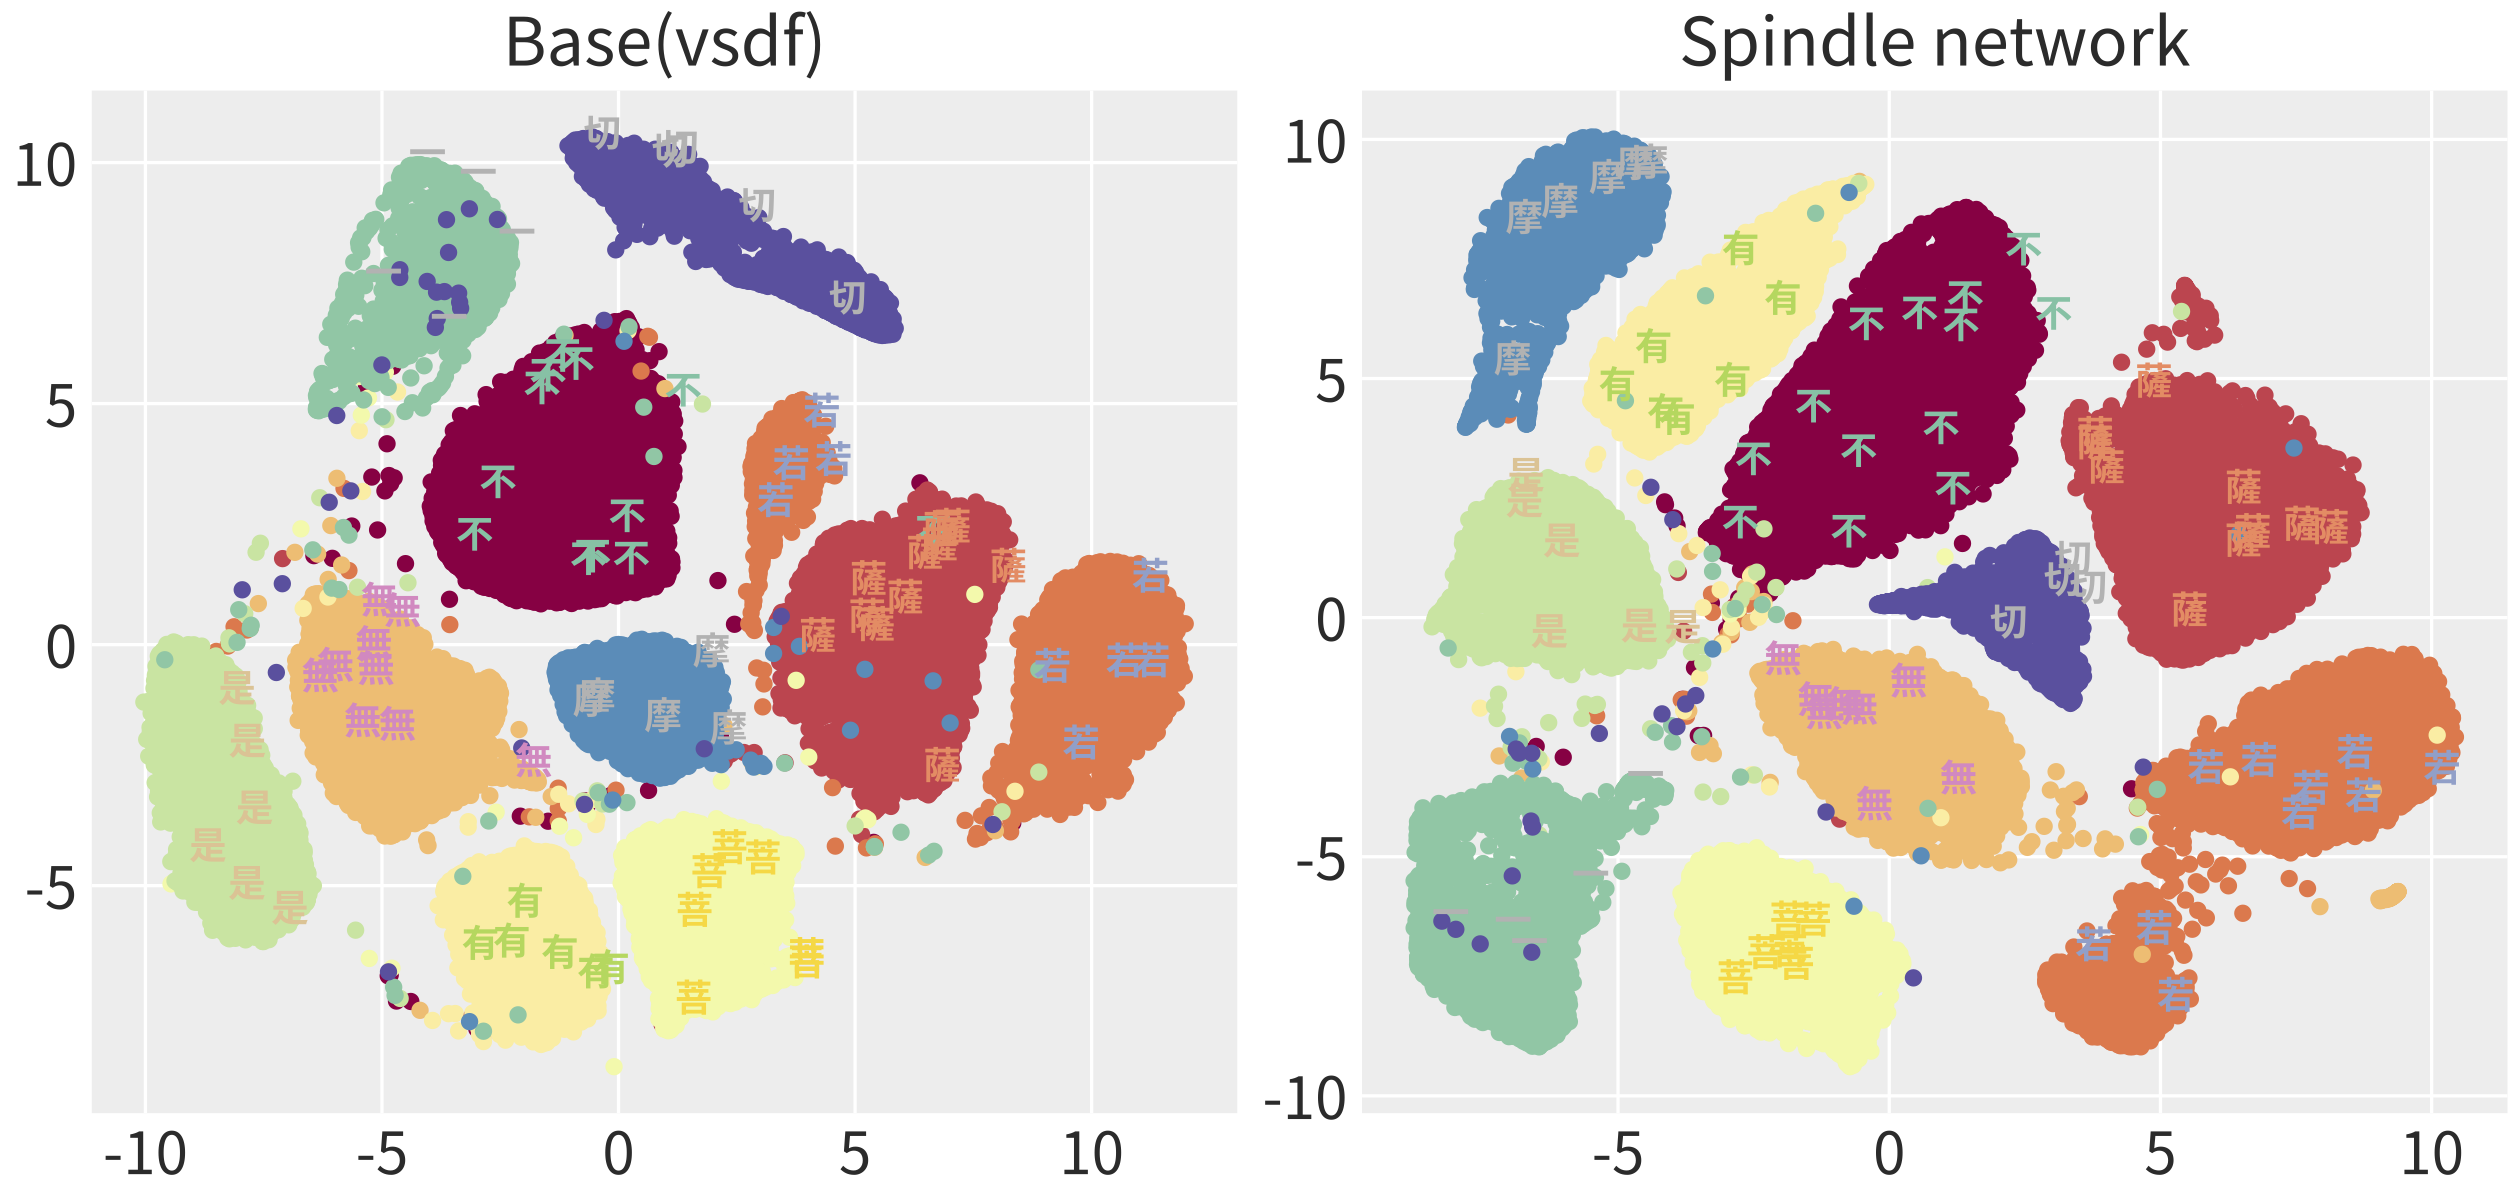
\includegraphics[width=1.0\linewidth]{figures/tsne.pdf}
    \end{center}
    \caption{Visualization of TSNE features from the top 10 character frequencies.}
    \label{fig:tsne}
\end{figure}

    
We further perform qualitative analysis to find out how the spindle net affects the character features, shown in Fig.\ref{fig:tsne}. In Fig.\ref{fig:tsne}, the tsne-cuda tool is used to visualize the last layer of features of the feature extractor. It can be seen that the features extracted by SpindleNet have clearer classification boundaries. For example, the orange character is divided into two  in base, while it is gathered together in SpindleNet. This shows that SpindleNet has better feature extraction capabilities.

\subsubsection{Architecture-level Ablative}
% In this section, we first demonstrate how the spindle-ness affects the performance. Then we discuss the structural sensitivity, i. e. which convolution layer deserves the most parameters. We first define the term ``spindle-ness'' by the largest channel number, % please change this one. and then perform quantitative analysis on the relation between the ``spindle-ness'' and the model performance.
% The results are shown in Fig.\ref{fig:spindleness}, ... % insert your analysis here.
\input{figures/archabl}
In this section, we discuss structural sensitivity, i.e.\ which convolutional layer deserves the most parameters. Fig.\ref{fig:archabl} shows the impact of structures on performance in two extreme cases, one is an equilateral triangle structure used in base, and the other is an inverted triangle structure. In the end, SpindleNet achieved the best results, which proves that appropriately increasing the number of channels or parameters in the head can improve model performance.

% We then analyze the structural sensitivity, i.e., which layer needs the most parameters. The results are shown in Fig.\ref{fig:archabl}. ... % insert your analysis here.


\section{Conclusion}
In this paper, we found that the similarity of character components can be exploited to improve performance in the tail of long-tail distribution data, which can improve the performance of new characters. 
Furthermore, We implemented a spindle network to enhance the ability to extract character component features, leveraging the similarities between character components to improve the recognition performance of new characters. Additional analysis demonstrates the effectiveness of SpindleNet.
Experiments on three challenging Chinese ancient book datasets (TKH, MTH1000, and MTH1200) to validate the superiority of our proposed method. The results show that our approach achieves state-of-the-art performance in this field.
In the future, we plan to train our framework in a weakly-supervised manner, which has proven to be successful in the scene text field.


\input{sec/6_acknowledgement}

%
% ---- Bibliography ----
%
% BibTeX users should specify bibliography style 'splncs04'.
% References will then be sorted and formatted in the correct style.
%
% \bibliographystyle{splncs04}
% \bibliography{mybibliography}
%

\bibliographystyle{splncs04}
\bibliography{ref/refs,ref/all.bib}

\end{document}
